\chapter{Тасклеты}

\section{Реализация}

\begin{lstlisting}[caption={}]
#include <linux/module.h>
#include <linux/kernel.h>
#include <linux/init.h>
#include <linux/interrupt.h>

#define HANDLED_IRQ 1

MODULE_LICENSE("GPL");
MODULE_AUTHOR("Faris Nabiev");

static int  __init my_tasklet_init(void);
static void __exit my_tasklet_exit(void);

module_init(my_tasklet_init);
module_exit(my_tasklet_exit);

static int dev_id;
const char *tasklet_data = "tasklet data";

// Функция обработки нижней половины
void tasklet_handler(unsigned long data);

// Регистрация тасклета
DECLARE_TASKLET(my_tasklet, tasklet_handler, (unsigned long)&tasklet_data);

void tasklet_handler(unsigned long data)
{
    printk(KERN_INFO "tasklet: state -- %ld, count -- %d, data -- %s\n",
           my_tasklet.state, atomic_read(&my_tasklet.count),
           (const char *)(*(unsigned long *)my_tasklet.data));
}

// Обработчик прерывания
static irqreturn_t ihandler(int irq, void *dev_id)
{
    // Проверка, что произошло именно нужное прервыние
    if (irq == HANDLED_IRQ)
    {
        printk(KERN_INFO "tasklet: scheduled\n");
        // Добавление тасклета в очередь
        tasklet_schedule(&my_tasklet);

        return IRQ_HANDLED; // Прерывание обработано
    }
    else
        return IRQ_NONE; // Прерывание не обработано
}

// Инициализация модуля
static int __init my_tasklet_init(void)
{
    // Совместное использование линии IRQ с другими устройствами
    if (request_irq(HANDLED_IRQ, ihandler, IRQF_SHARED,
                    "ihandler", &dev_id))
    {
        printk(KERN_ERR "tasklet: Error on request_irq\n");

        return -1;
    }

    printk(KERN_INFO "tasklet: Module loaded!\n");

    return 0;
}

// Выгрузка модуля
static void __exit my_tasklet_exit(void)
{
    // Удаление тасклета
    tasklet_disable(&my_tasklet);
    tasklet_kill(&my_tasklet);
    // Освобождение линии прерывания
    free_irq(HANDLED_IRQ, &dev_id);

    printk(KERN_INFO "tasklet: Module unloaded!\n");
}
\end{lstlisting}

\section{Результаты работы}

\begin{figure}[H]
    \centering
    \caption{Сборка}
    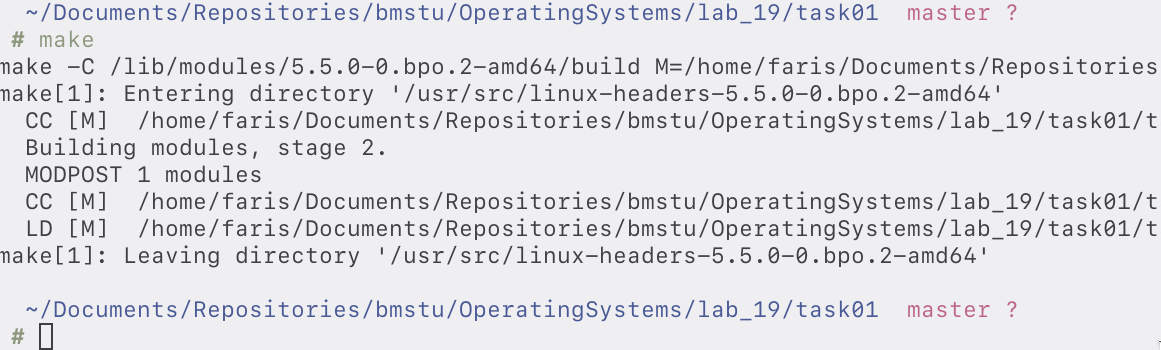
\includegraphics[scale=0.375]{images/scr1_1.png}
\end{figure}
\begin{figure}[H]
    \centering
    \caption{Загрузка модуля ядра, вывод буфера сообщений ядра, проверка списка загруженных модулей}
    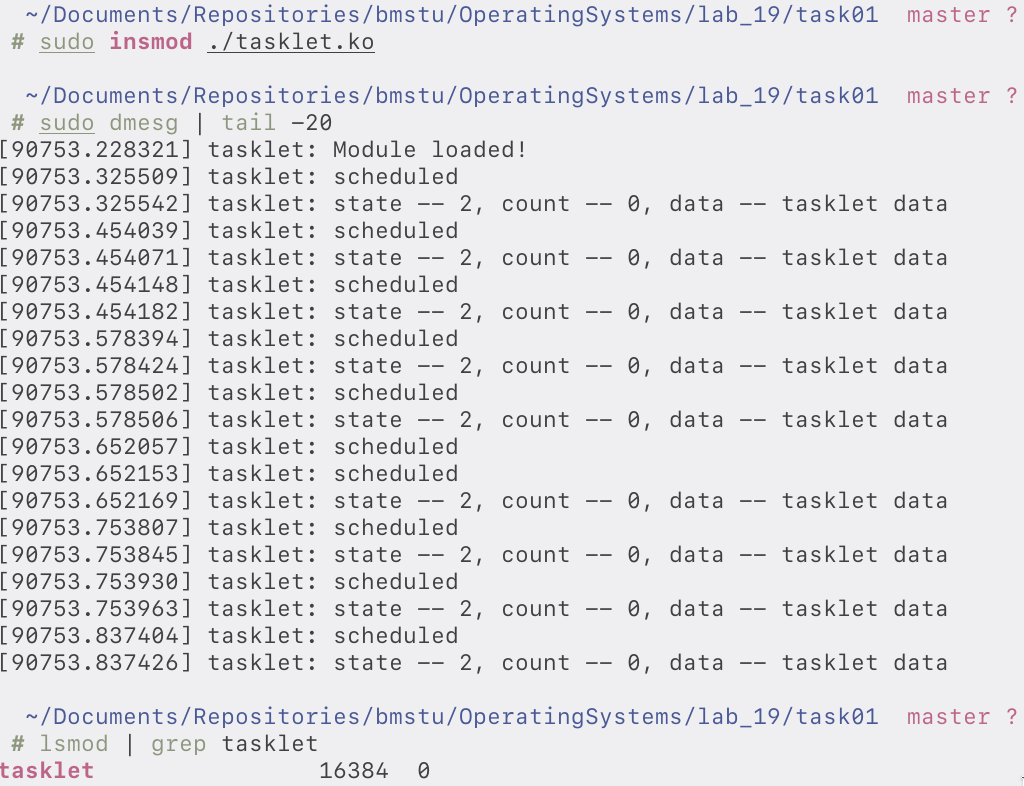
\includegraphics[scale=0.375]{images/scr1_2.png}
\end{figure}
\begin{figure}[H]
    \centering
    \caption{Просмотр содержимого /proc/interrupts}
    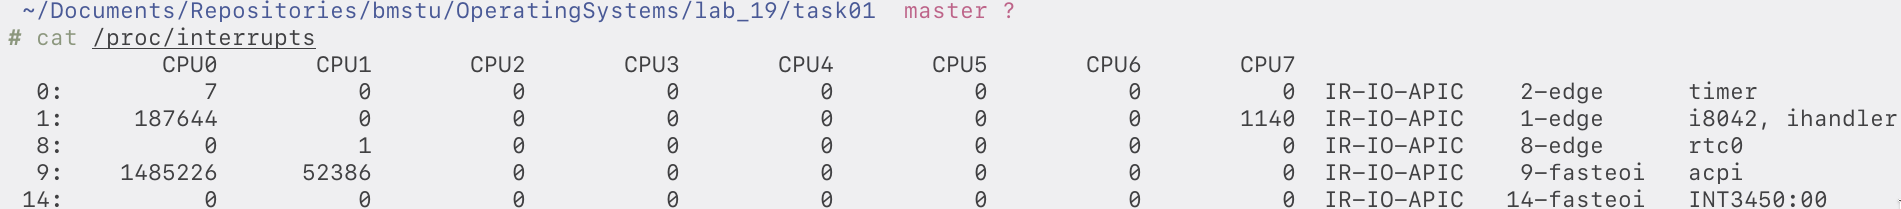
\includegraphics[scale=0.235]{images/scr1_3.png}
\end{figure}
\begin{figure}[H]
    \centering
    \caption{Выгрузка модуля ядра, вывод буфера сообщений ядра}
    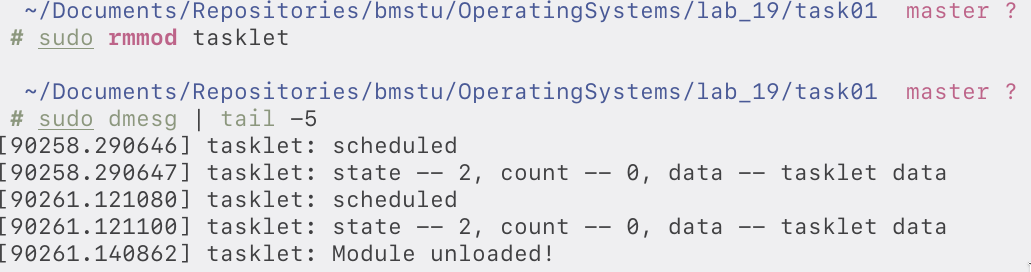
\includegraphics[scale=0.375]{images/scr1_4.png}
\end{figure}
